\documentclass[11pt]{article}

\usepackage{amsmath, amsthm, amssymb}
\usepackage[hidelinks]{hyperref}
\usepackage{geometry}
\geometry{margin=1in}
\usepackage{authblk}
\usepackage{graphicx}

\newtheorem{theorem}{Theorem}
\newtheorem{lemma}[theorem]{Lemma}
\newtheorem{corollary}[theorem]{Corollary}
\newtheorem{definition}[theorem]{Definition}
\newtheorem{remark}[theorem]{Remark}

\newcommand{\bfa}{\mathbf{a}}
\newcommand{\bfb}{\mathbf{b}}
\newcommand{\intro}{\mathrm{intro}}
\newcommand{\pC}{p_C^{\intro}}

\title{An Exact Cooperation Formula for Introspection Dynamics in the Heterogeneous Public Goods Game}
\author[1]{Harry Foster}
\author[1]{Vince Knight}
\author[2]{Sebastian Krapohl}
\affil[1]{School of Mathematics, Cardiff University}
\affil[2]{Faculty of Social and Behavioural Sciences, University of Amsterdam}
\date{\today}

\begin{document}

\maketitle

\begin{abstract}
We study introspection dynamics on the heterogeneous public goods game, where \(N\) players
may differ in their contributions \(\alpha_i\), public goods multipliers \(r_i\), and choice
intensities \(\beta_i\). We prove that the payoff difference a player evaluates
when considering a strategy switch is independent of all other players' current actions, a
consequence of the linear payoff structure. This state-independence implies that the introspection
Markov chain decomposes as a random-scan product of \(N\) independent two-state chains, one
per player. The stationary distribution is therefore a product measure, and the long-run
cooperation probability admits the exact closed form
\[
  \pC = \frac{1}{N}\sum_{i=1}^{N}
        \left[\frac{1-2\mu_i}{1+e^{\,\beta_i\alpha_i(1-r_i/N)}}+\mu_i\right],
\]
with no asymptotic approximation. Several structural consequences follow immediately:
a player-specific cooperation threshold at \(r_i = N\), neutrality under zero choice
intensity, and the sign of each player's sensitivity to their own parameters.
\end{abstract}

\section{Introduction}

The public goods game is a canonical model of cooperation in evolutionary game theory:
players decide whether to contribute to a common resource, which is multiplied and
redistributed equally, creating a tension between individual incentive and collective
benefit~\cite{nowak2006five}. Classical analyses assume a homogeneous population, but
real groups are heterogeneous: players differ in their productivity, their contributions,
and how sensitively they respond to payoff differences~\cite{hauser2019social}.

A natural learning rule for such settings is \emph{introspection dynamics}, introduced
in~\cite{couto2022introspection}: at each time step a player
compares their current payoff to the payoff they \emph{would have received} had they
played the alternative action (keeping all other players fixed), and switches with a
probability governed by this difference. Because the comparison is
self-referential rather than imitative, introspection applies to arbitrary asymmetric
games where role-model imitation is unavailable or unnatural.

In~\cite{couto2023multiplayer} the authors extended introspection dynamics to multiplayer
asymmetric games and derived a formula for the stationary distribution that can be
evaluated numerically for any game. In their general framework the transition rate for
player \(i\) switching depends on the actions of all other players through the payoff
function, so the stationary distribution must be computed by solving a linear system of
dimension \(2^N\); no closed form is available in general.

In this paper we show that the specific payoff structure of the heterogeneous public
goods game admits an exact closed-form analysis. The key observation is that the
payoff difference \(\Delta\pi_i\) a player evaluates depends only on their
own current action and individual parameters, not on the actions of others. This is a consequence of the
\emph{linearity} of the public goods payoff in contributions. As a result, the
introspection chain decomposes exactly as a product of \(N\) independent two-state chains
(one per player), the stationary distribution is a product measure, and the cooperation
probability \(\pC\) admits an explicit closed form that scales as \(O(N)\) rather than
\(O(2^N)\).

The paper is organised as follows. Section~\ref{sec:setup} introduces the model.
Section~\ref{sec:payoff} establishes the payoff identity. Section~\ref{sec:decomp}
proves the product decomposition and derives the exact cooperation formula.
Section~\ref{sec:consequences} records several structural corollaries.
Section~\ref{sec:conclusion} concludes.

\section{Setup and notation}\label{sec:setup}

Consider a well-mixed population of \(N\) ordered players with contributions
\(\alpha_1,\ldots,\alpha_N>0\), player-specific public goods multipliers
\(r_1,\ldots,r_N>1\), player-specific choice intensities \(\beta_1,\ldots,\beta_N>0\),
and two actions \(\{C,D\}\) coded as \(\{1,0\}\). The state space is
\(S=\{0,1\}^N\) with \(|S|=2^N\).

\textbf{Payoff.} The payoff to player \(i\) in state \(\bfa=(a_1,\ldots,a_N)\) is

\begin{equation}\label{eq:payoff}
  \pi_i(\bfa) = \frac{r_i}{N}\sum_{j=1}^N \alpha_j a_j - \alpha_i a_i.
\end{equation}

We write \(C(\bfa)=\sum_j\alpha_j a_j\) for the total contribution.

To give the definition of introspection dynamics we define the following two
quantities.

\textbf{Fermi function.} Each player \(i\) has a personal Fermi function
\(\phi_i(x)=(1+e^{\beta_i x})^{-1}\). Since \(\beta_i>0\), the exponential
\(e^{\beta_i x}\) is strictly increasing in \(x\), so \(\phi_i\) is strictly
decreasing with \(\phi_i(0)=\tfrac{1}{2}\) and \(\phi_i(x)+\phi_i(-x)=1\).

\textbf{Mutation.} Each player \(i\) has a mutation rate
\(\mu_i \in(0,\tfrac{1}{2})\), ensuring ergodicity of the Markov chain. This is
the probability with which they mutate to the other action regardless of the
intended choice of the dynamic.


\begin{definition}[Cooperation probability]
Given an ergodic chain on \(S\) with stationary distribution \(\pi\), the
\emph{cooperation probability} is \(p_C=\pi\cdot s\), where
\(s_\bfa=\frac{1}{N}\sum_i a_i\) is the fraction of cooperators in state \(\bfa\).
\end{definition}

\textbf{Introspection dynamics.} At each step, one player \(i\) is selected
uniformly at random. Player \(i\) considers switching from action \(a_i\) to the
alternative \(\bar{a}_i=1-a_i\). Writing \(\bfa_{i\to\bar{a}_i}\) for the state
obtained by flipping only coordinate \(i\), the transition probability for the
switch is

\begin{equation}\label{eq:intro-transition}
  T^{\intro}_{\bfa,\,\bfa_{i\to\bar{a}_i}}
  = \frac{1}{N}\bigl[\phi_i(\Delta\pi_i)(1-2\mu_i)+\mu_i\bigr],
\end{equation}

where \(\Delta\pi_i:=\pi_i(\bfa)-\pi_i(\bfa_{i\to\bar{a}_i})\) is the
payoff gain from keeping action \(a_i\). Since \(\phi_i\) is
strictly decreasing, a larger payoff gain from the current action yields a
smaller switching probability.

\section{The payoff identity}\label{sec:payoff}

\begin{lemma}[State-independence of payoff differences]
\label{lem:payoff-identity}

For the payoff~\eqref{eq:payoff}, the difference player \(i\)
evaluates when considering a switch from \(a_i\) to \(\bar{a}_i\) is
\begin{equation}\label{eq:delta-pi}
  \Delta\pi_i = (2a_i-1)\,\alpha_i\!\left(\frac{r_i}{N}-1\right).
\end{equation}
This depends only on \(a_i\), \(\alpha_i\), \(r_i\), and \(N\); in particular, it is
independent of all other players' actions \(\bfa_{-i}\).
\end{lemma}

\begin{proof}
When player \(i\) switches from \(a_i\) to \(\bar{a}_i=1-a_i\), only their own
contribution changes, so the total contribution becomes
\(C(\bfa_{i\to\bar{a}_i}) = C(\bfa)+\alpha_i(1-2a_i)\).
Expanding both payoffs:
\begin{align*}
  \pi_i(\bfa) &= \frac{r_i}{N}\,C(\bfa)-\alpha_i a_i, \\
  \pi_i(\bfa_{i\to\bar{a}_i})
  &= \frac{r_i}{N}\bigl[C(\bfa)+\alpha_i(1-2a_i)\bigr]-\alpha_i(1-a_i).
\end{align*}

Subtracting:

\begin{align*}
  \Delta\pi_i
  &= -\frac{r_i}{N}\alpha_i(1-2a_i) + \alpha_i(1-2a_i) \\
  &= \alpha_i(1-2a_i)\!\left(1-\frac{r_i}{N}\right) \\
  &= \alpha_i(2a_i-1)\!\left(\frac{r_i}{N}-1\right).
\end{align*}

The term \(C(\bfa)\) cancels entirely, so \(\Delta\pi_i\) is
independent of \(\bfa_{-i}\).

\end{proof}

\begin{remark}

The cancellation of \(C(\bfa)\) relies on the payoff~\eqref{eq:payoff} being
\emph{linear} in contributions. The heterogeneity of \(r_i\) does not affect this
cancellation: each player's comparison depends only on their own
parameters.

\end{remark}

\section{Individual cooperation probabilities}\label{sec:decomp}

By Lemma~\ref{lem:payoff-identity}, player \(i\)'s update depends only on their own
action \(a_i\), not on \(\bfa_{-i}\). We use this to compute each player's long-run
cooperation probability directly from their two-state update rule.

\begin{theorem}[Individual cooperation probabilities]\label{thm:decomp}

Under introspection dynamics with player-specific \(\beta_i\) and \(r_i\), uniform
mutation \(\mu_i\in(0,\tfrac{1}{2})\), and payoff~\eqref{eq:payoff}, the long-run
probability that player \(i\) cooperates is

\begin{align}
  p_i &= \phi_i\!\bigl(\alpha_i(1-r_i/N)\bigr)(1-2\mu_i)+\mu_i. \label{eq:pi}
\end{align}
\end{theorem}

\begin{proof}

By Lemma~\ref{lem:payoff-identity}, \(\Delta\pi_i\) depends only on \(a_i\). When
player \(i\) is selected, the probability their next action is \(C\) equals \(p_i\)
regardless of their current action: if \(a_i=D\), the switch probability is
\(\phi_i(\alpha_i(1-r_i/N))(1-2\mu_i)+\mu_i=p_i\); if \(a_i=C\), the probability of
remaining at \(C\) is \(1-[\phi_i(\alpha_i(r_i/N-1))(1-2\mu_i)+\mu_i]=p_i\), using
\(\phi_i(x)+\phi_i(-x)=1\). Since each selection of player \(i\) places them in state
\(C\) with probability \(p_i\) independently of their current state, the long-run
cooperation probability of player \(i\) is \(p_i\).

\end{proof}

\begin{corollary}[Exact cooperation probability]\label{cor:exact-pC}

The long-run cooperation probability is

\begin{equation}\label{eq:pC}
  \boxed{
  \pC = \frac{1}{N}\sum_{i=1}^{N}
        \left[\frac{1-2\mu_i}{1+e^{\,\beta_i\alpha_i(1-r_i/N)}}+\mu_i\right].
  }
\end{equation}

\end{corollary}

\begin{proof}

By Theorem~\ref{thm:decomp}: 

\[
  \pC = \frac{1}{N}\sum_{i=1}^N p_i.
\]
Substituting \(\phi_i(\alpha_i(1-r_i/N))=(1+e^{\beta_i\alpha_i(1-r_i/N)})^{-1}\)
into~\eqref{eq:pi} gives~\eqref{eq:pC}.

\end{proof}

\begin{figure}[ht]
  \centering
  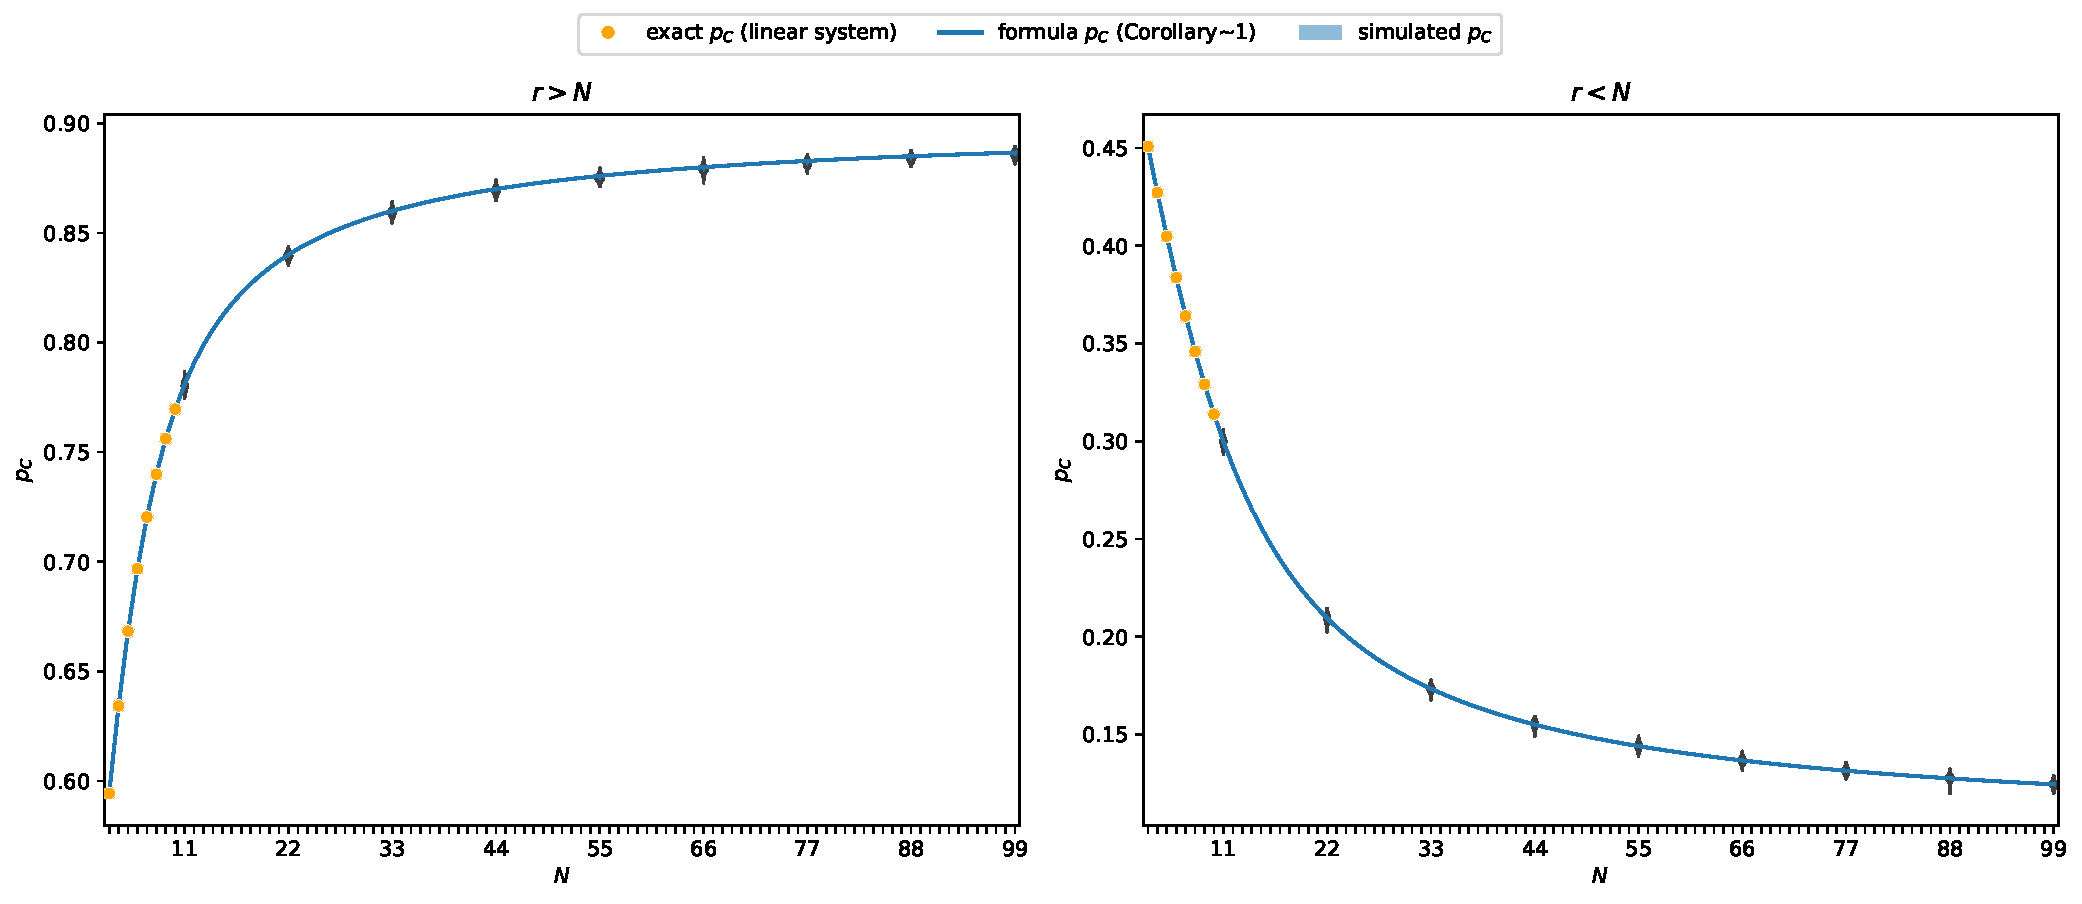
\includegraphics[width=\textwidth]{../assets/graphs/simulations/main.pdf}
  \caption{Validation of the exact formula~\eqref{eq:pC} on a heterogeneous group
    with contributions \(\alpha_i = i\) for \(i = 0, 1, \ldots, N-1\), choice
    intensity \(\beta = 0.5\), and mutation rate \(\mu_i = 0.1\).
    \textit{Left:} \(r = 2N\) (so \(r > N\) for all \(N\)).
    \textit{Right:} \(r = N/2\) (so \(r < N\) for all \(N\)).
    Orange dots: exact \(p_C\) obtained by solving the full \(2^N\) linear system
    (feasible only for small \(N\)).
    Blue curve: the closed-form formula~\eqref{eq:pC} (Theorem~\ref{thm:decomp}).
    Blue bands: cooperation probability estimated from \(10^5\) simulation steps
    across 99 independent runs; the band width reflects run-to-run variability.
    The exact and the estimated values of \(p_C\) are obtained
    using~\cite{harry_foster_2026_19495532}.
    The formula matches both the exact values and the simulations exactly.}
  \label{fig:validation}
\end{figure}

\section{Structural consequences}\label{sec:consequences}

The closed form~\eqref{eq:pC} allows immediate structural conclusions about how
cooperation depends on game parameters.

\begin{corollary}[Player-specific cooperation thresholds]\label{cor:threshold}
    
Player \(i\) cooperates with probability greater than \(\frac{1}{2}\) if and only if
\(r_i > N\). A sufficient condition for \(\pC > \tfrac{1}{2}\) is \(r_i > N\) for all \(i\).

\end{corollary}

\begin{proof}
    
Since \(\phi_i\) is strictly decreasing with \(\phi_i(0)=\tfrac{1}{2}\):
\[
  p_i > \tfrac{1}{2}
  \iff \phi_i\!\bigl(\alpha_i(1-r_i/N)\bigr) > \tfrac{1}{2}
  \iff \alpha_i(1-r_i/N) < 0
  \iff r_i > N.
\]

The average \(\pC=\frac{1}{N}\sum_i p_i\) exceeds \(\tfrac{1}{2}\) whenever every
summand does.

\end{proof}

\begin{corollary}[Neutral drift]\label{cor:neutral}

If \(\beta_i=0\) for all \(i\), then \(\pC=\tfrac{1}{2}\) regardless of all other
parameters.

\end{corollary}

\begin{proof}

When \(\beta_i=0\), the Fermi function satisfies \(\phi_i(x)=\tfrac{1}{2}\) for all \(x\).
Substituting into~\eqref{eq:pC}:
\[
  \pC = \frac{1}{N}\sum_{i=1}^N\left[\frac{1-2\mu_i}{2}+\mu_i\right]
       = \frac{1-2\mu_i}{2}+\mu_i = \frac{1}{2}.\qedhere
\]

\end{proof}

\begin{corollary}[Role of heterogeneity]\label{cor:heterogeneity}

For player \(i\) with \(r_i\neq N\):

\begin{enumerate}
  \item[(i)] \(\dfrac{\partial p_i}{\partial\alpha_i}\) is positive when \(r_i>N\) and
             negative when \(r_i<N\).
  \item[(ii)] \(\dfrac{\partial p_i}{\partial\beta_i}\) is positive when \(r_i>N\) and
              negative when \(r_i<N\).
\end{enumerate}

\end{corollary}

\begin{proof}

Write \(p_i=(1-2\mu_i)\phi_i(\alpha_i(1-r_i/N))+\mu_i\).

\textit{Part (i).} Differentiating with respect to \(\alpha_i\):
\[
  \frac{\partial p_i}{\partial\alpha_i}
    = (1-2\mu_i)(1-r_i/N)\,\phi_i'(\alpha_i(1-r_i/N)).
\]
Since \(\phi_i'(x)<0\) for all \(x\) and \(1-2\mu_i>0\), the sign equals
\(-\mathrm{sgn}(1-r_i/N)=\mathrm{sgn}(r_i/N-1)\), which is positive if and only
    if\(r_i>N\).

\textit{Part (ii).} Write \(g(t)=(1+e^t)^{-1}\), so \(\phi_i(x)=g(\beta_i x)\).
Differentiating with respect to \(\beta_i\):
\[
  \frac{\partial p_i}{\partial\beta_i}
    = (1-2\mu_i)\,\alpha_i(1-r_i/N)\,g'(\beta_i\alpha_i(1-r_i/N)).
\]
Since \(g'<0\) and \(\alpha_i>0\), the sign equals
\(-\mathrm{sgn}(1-r_i/N)=\mathrm{sgn}(r_i/N-1)\), which is positive if and only
    if \(r_i>N\).
\end{proof}

\begin{remark}

Corollaries~\ref{cor:threshold}--\ref{cor:heterogeneity} show that each player's
long-run cooperation is fully determined by their individual triple \((\alpha_i,\beta_i,r_i)\)
and the group size \(N\). Players with \(r_i>N\) cooperate more than half the time, and increasing
\(\alpha_i\) or \(\beta_i\) raises their cooperation probability further; players
with \(r_i<N\) show the opposite sensitivity. The parameters of other
players have no effect on player \(i\)'s marginal cooperation probability.

\end{remark}

\begin{figure}[ht]
  \centering
  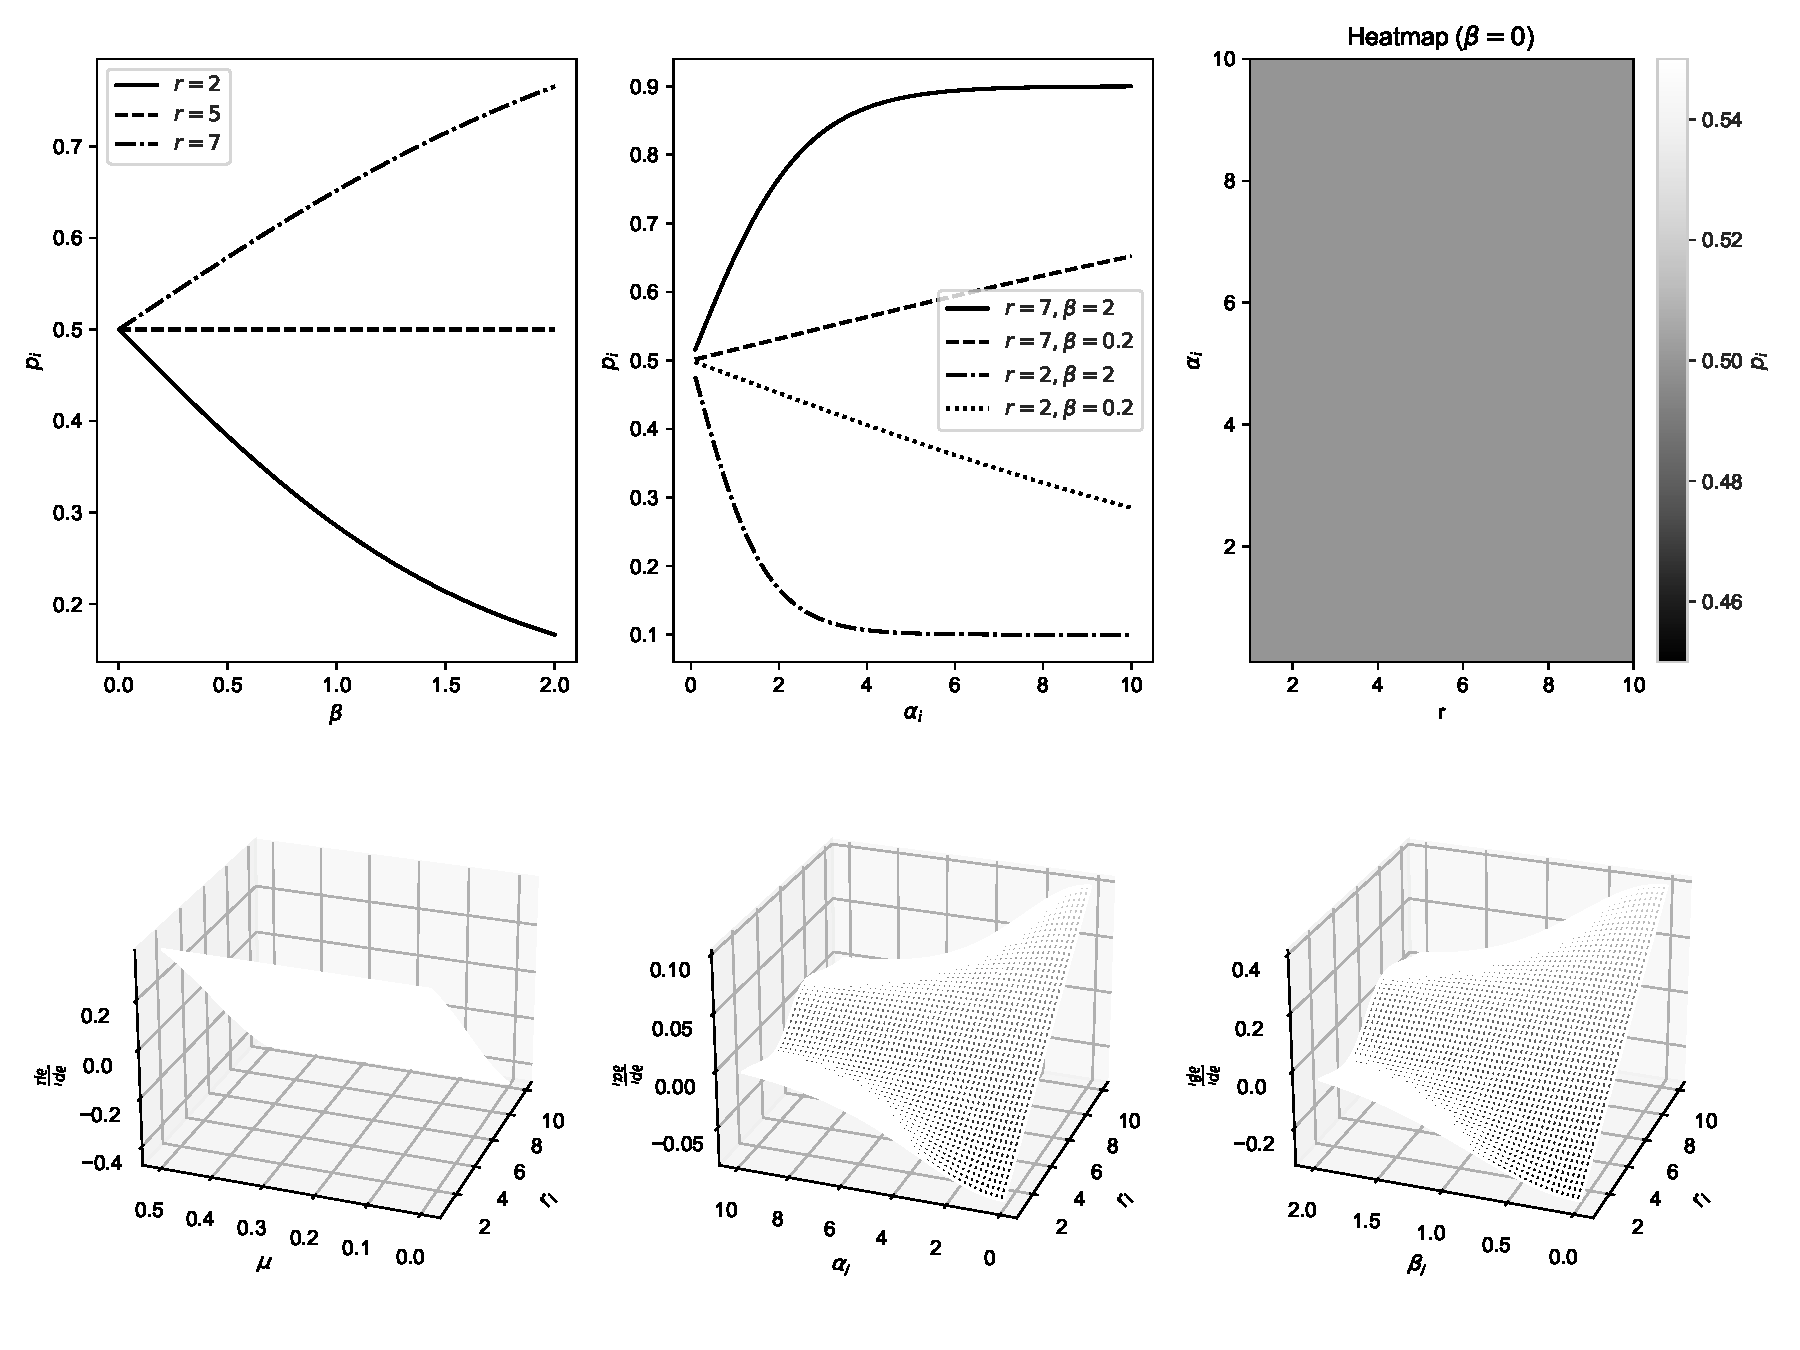
\includegraphics[width=\textwidth]{../assets/graphs/big_panel/main.pdf}
  \caption{Structural properties of \(p_i\) for a single player with \(N = 5\),
    \(\mu_i = 0.1\).
    \textit{Top left:} \(p_i\) as a function of \(\beta_i\) (\(\alpha_i = 2\))
    for \(r < N\), \(r = N\), and \(r > N\); all curves pass through \(p_i = \tfrac{1}{2}\)
    at \(\beta_i = 0\) (Corollary~\ref{cor:neutral}).
    \textit{Top centre:} \(p_i\) as a function of \(\alpha_i\) for two values of
    \(r\) and \(\beta_i\); curves above (below) \(\tfrac{1}{2}\) correspond to
    \(r > N\) (\(r < N\)).
    \textit{Top right:} \(p_i(\alpha_i, r_i)\) at \(\beta_i = 0\), confirming
    \(p_i = \tfrac{1}{2}\) everywhere (Corollary~\ref{cor:neutral}); the dashed
    line marks \(r_i = N\).
    \textit{Bottom row:} Heatmaps of the partial derivatives
    \(\partial p_i/\partial \mu_i\), \(\partial p_i/\partial \alpha_i\), and
    \(\partial p_i/\partial \beta_i\) over the \((r_i, \alpha_i)\) or
    \((r_i, \beta_i)\) plane (\(\beta_i = 0.5\) or \(\alpha_i = 2\) as fixed
    parameter). Red indicates a positive derivative; blue indicates negative.
    Each derivative changes sign exactly at \(r_i = N\) (dashed line), consistent
    with Corollary~\ref{cor:heterogeneity}.}
  \label{fig:panel}
\end{figure}

\section{Conclusion}\label{sec:conclusion}

We have proved that introspection dynamics on the heterogeneous public goods game is
exactly solvable. The linear payoff structure implies that each player's payoff comparison
is independent of all other players' actions (Lemma~\ref{lem:payoff-identity}), so when
player \(i\) is selected their next action is \(C\) with probability \(p_i\) regardless
of current state (Theorem~\ref{thm:decomp}). The long-run cooperation probability
therefore has a closed form with \(N\) terms rather than \(2^N\)
(Corollary~\ref{cor:exact-pC}).

\newpage
\bibliographystyle{plain}
\bibliography{bibliography}

\end{document}
